\section*{What's Version Control? Why am I doing this?}

When you write a document, you have a few basic steps: you start the document and save, revise the document and save then finally publish the document.  But, you repeat the second step many times.

Here's the problem, as you revise the document, your previous versions are lost (or at a minimum difficult to access).  So, what do you do?  A lot of people start doing ``ad-hoc" version control.  You might create duplicates of the file at certain points, or put a previous version of a paragraph in a comment or depend on in-application versioning.  None of these are particularly satisfactory and tend to make more of mess than anything else.

Now, as messy as ``ad-hoc" versioning is with one person, it is far worse when you have multiple authors.  Consider a paper with three authors (figure \ref{fig:timeline}).  Some authors might make a large number of changes in a short period of time, others take a long period of time to do less edits.  And these edit periods overlap.  If you were doing this Word and E-Mail, this would result in multiple versions of the document that then would have to be hand merged. Not so with LaTeX and Git.

\begin{figure}[hbt]
	\centering
  	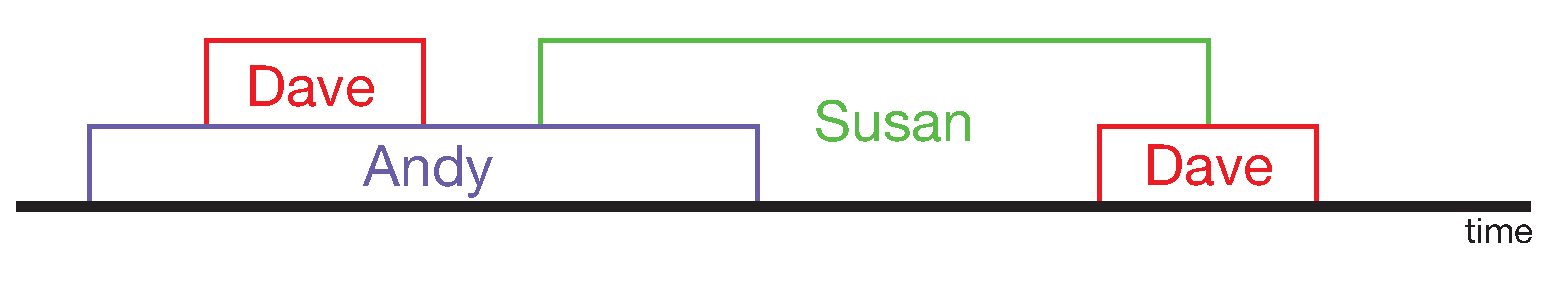
\includegraphics[width=6in]{graphics/timeline.eps}
  	\caption{Some edits take different periods of time and the edits overlap}
  	\label{fig:timeline}
\end{figure}